% paper_prd_inclusive.tex -- Article: the inclusive measurement.
% Companion of paper_prl_proton_tagged.tex (joint submission). No length limit.
\documentclass[aps,prd,twocolumn,superscriptaddress,nofootinbib,floatfix]{revtex4-2}
\usepackage{amsmath,amssymb}
\usepackage{graphicx}
\usepackage{booktabs}
\usepackage{xcolor}
\usepackage{hyperref}
\graphicspath{{figures/}{figures/bkgfit/}}
% Shared macros for the two papers. Kept identical to the analysis note's definitions.
\newcommand{\numu}{$\nu_\mu$}
\newcommand{\numubar}{$\bar{\nu}_\mu$}
\newcommand{\ccpip}{$\mathrm{CC}\pi^{\pm}$}
\newcommand{\uboone}{MicroBooNE}
\newcommand{\GeVc}{\,\text{GeV}\!/c}
\newcommand{\pot}{\,\text{POT}}
\newcommand{\pmuM}{p_\mu}
\newcommand{\ppiM}{p_\pi}
\newcommand{\cthmuM}{\cos\theta_\mu}
\newcommand{\cthpiM}{\cos\theta_\pi}
\newcommand{\thmupM}{\theta_{\mu\pi}}
\newcommand{\AC}{A_C}
% Draft status. Every data point in both papers is a Poisson throw of the central-value
% simulation: the signal region is blind. FHC and combined normalisations are being rebuilt on
% the corrected Run-1 exposure and the numbers here predate that rebuild.
\newcommand{\draftbanner}{\begin{center}\fbox{\parbox{0.95\linewidth}{\small\textbf{DRAFT ---
  blind analysis.} Every ``data'' point is a Poisson throw of the central-value simulation. Numbers
  are placeholders for the unblinded result; FHC and combined normalisations predate the Run-1
  exposure correction and will move by $\approx\!+14\%$ and $+6\%$.}}\end{center}}


\begin{document}

\title{Measurement of $\nu_\mu$ and $\bar\nu_\mu$ charged-current single charged-pion production
  differential cross sections on argon in the NuMI beam with the \uboone{} detector}

\author{The \uboone{} Collaboration}
\noaffiliation

\date{\today}

\begin{abstract}
We report flux-averaged total and differential cross sections for charged-current
single-charged-pion production, $\nu_\mu(\bar\nu_\mu)\,\mathrm{Ar}\to\mu^\mp\pi^\pm X$ with no
neutral pion in the final state, measured with the \uboone{} liquid-argon time-projection chamber
using its full exposure to the off-axis NuMI beam: $8.86\times10^{20}$ protons on target in forward
horn current, $1.11\times10^{21}$ in reverse horn current, and their combination. Each
configuration is an independent measurement with its own flux, and all angles are defined about the
neutrino direction, which lies $28^\circ$ from the detector axis. Differential cross sections are
extracted by Wiener-SVD unfolding in muon momentum, pion momentum, muon polar angle in two
parameterisations, pion polar angle and the muon--pion opening angle, and the total from a one-bin
extraction of the same machinery; every result is released with its additional-smearing matrix and
full covariance. The implementation, the statistical uncertainties and the robustness of the
extraction to a materially different interaction model are validated on simulation, and the
background model is tested in four control regions opened on beam-on data. The results are compared
with GENIE, NuWro, NEUT and GiBUU. [DRAFT: values are blind placeholders.]
\end{abstract}

\maketitle
\draftbanner

\section{Introduction}

Charged-current single charged-pion production,
$\nu_\mu(\bar\nu_\mu)+\mathrm{Ar}\to\mu^\mp+\pi^\pm+X$, is among the most frequent neutrino
interactions between $1$ and $5$~GeV and is a leading background to $\nu_e$ appearance
measurements at NOvA~\cite{nova}, T2K~\cite{t2k} and DUNE~\cite{dune}. Its cross section on
nuclear targets is not well constrained: the generators used by those experiments disagree by
$20$--$30\%$ in rate and more in shape. On argon it has been measured in the NuMI beam by
ArgoNeuT~\cite{argoneut_ccpi} with a sample of tens of events, and by \uboone{} in the Booster
Neutrino Beam~\cite{uboone_bnb2026_ccpi}; the $\nu_e$ channel has been measured by \uboone{} in
NuMI~\cite{uboone_nue_ccpi}.

This article presents the $\nu_\mu+\bar\nu_\mu$ measurement with the full \uboone{} NuMI exposure,
in three configurations: forward horn current (FHC), reverse horn current (RHC), and their
combination. The NuMI beam at \uboone{}'s off-axis location differs from the Booster beam in
energy, composition and direction, and the reverse-horn running supplies an antineutrino-enriched
sample in the same detector. A companion Letter~\cite{companion_prl} reports the kinematics of the
hadronic system in the subsample with a reconstructed proton.

The measurement is built in five steps and the article follows them: the exposure and flux
(\S\ref{sec:flux}); the signal definition and selection (\S\ref{sec:signal}--\ref{sec:selection});
the response and unfolding (\S\ref{sec:unfolding}); the uncertainties (\S\ref{sec:syst}); and the
validation and control regions (\S\ref{sec:validation}--\ref{sec:cr}). The results are in
\S\ref{sec:results}.

\section{Beam, exposure and flux}
\label{sec:flux}

\uboone{}~\cite{uboone_nim} is an $85$-tonne active-mass LArTPC at Fermilab, $135$~mrad off the
axis of the NuMI beam~\cite{numi_beam} at $673$~m from the target. In FHC the flux at the detector
is $\nu_\mu$-dominated; in RHC the $\bar\nu_\mu$ fraction is substantially enhanced, and the
$\nu_\mu+\bar\nu_\mu$ integral is lower because the reverse-horn focusing accepts a softer hadron
spectrum at the off-axis location. Both flavours are signal in every configuration.

\begin{table}[b]
  \caption{Exposure and integrated $\nu_\mu+\bar\nu_\mu$ flux above $60$~MeV per configuration.
    [DRAFT: FHC and combined exposures predate the Run-1 correction, which reduces FHC to
    $7.77\times10^{20}$ and the combined to $1.88\times10^{21}$.]}
  \label{tab:exposure}
  \begin{ruledtabular}
  \begin{tabular}{lcc}
    Configuration & POT & $\Phi$ [$10^{-10}$~cm$^{-2}$~POT$^{-1}$] \\
    \hline
    FHC (Runs 1, 2, 4, 5) & $8.857\times10^{20}$ & $6.81159$ \\
    RHC (Runs 1, 2, 3, 4) & $11.082\times10^{20}$ & $6.44646$ \\
    Combined & $19.939\times10^{20}$ & $6.60865$ \\
  \end{tabular}
  \end{ruledtabular}
\end{table}

The exposure is normalised run period by run period: each period's simulation is scaled to that
period's delivered protons on target and its beam-off sample to that period's ratio of beam-on to
beam-off gates, because the per-period factors differ by up to a factor of two and a pooled factor
would misweight the detector conditions that the response has to represent. The integrated flux of
each configuration (Table~\ref{tab:exposure}) is taken from the PPFX-corrected NuMI flux
simulation~\cite{ppfx}, and the combined configuration's flux is the exposure-weighted mean.

\subsection{The neutrino direction}
\label{sec:beamdir}

At an off-axis detector the neutrino direction is not the detector $z$ axis: at \uboone{} it lies
$28^\circ$ away, from the NuMI target to the detector. Every polar angle and every transverse
quantity in this article is defined about the neutrino direction --- at truth level the exact
per-event direction, at reconstruction level the direction from the target to the reconstructed
vertex, which coincides with the per-event direction to a fraction of a degree. The difference is
not cosmetic: computed about the detector axis, $65\%$ of signal events fall in a different
$\cos\theta_\mu$ bin, and the transverse-imbalance variables of the companion Letter change by
factors of two to three.

\section{Simulation}
\label{sec:mc}

Neutrino interactions are generated with GENIE~v3~\cite{genie,genie3} with the \uboone{}
tune~\cite{uboone_tune}, propagated with GEANT4, overlaid on beam-off data to model cosmic
activity, and reconstructed with Pandora~\cite{pandora,uboone_pandora}. Cosmic-only backgrounds
use a dedicated beam-off sample per run period; interactions outside the cryostat use a dirt
sample. Systematic universes for the flux (PPFX multisims), the interaction model (GENIE multisims
and unisims) and hadron re-interaction (GEANT4 reweighting) are stored per event; detector-response
variations use dedicated samples~\cite{uboone_detvar}. Four standalone generators are compared with
the results: GENIE~v3, NuWro~\cite{nuwro}, NEUT~\cite{neut,neut2021} and GiBUU~\cite{gibuu}, each
run with the NuMI flux of the corresponding configuration.

\section{Signal definition}
\label{sec:signal}

The signal is defined by the particles leaving the nucleus, not by the interaction mechanism: a
$\nu_\mu$ or $\bar\nu_\mu$ charged-current interaction with a true vertex inside the fiducial
volume, exactly one muon with $p_\mu>0.15\GeVc$, exactly one charged pion with $p_\pi>0.175\GeVc$,
no $\pi^0$ and no other meson, any number of nucleons, and a muon--pion opening angle
$\theta_{\mu\pi}<2.6$~rad. Coherent pion production satisfies this definition and is signal.
Final-state interactions --- pion absorption, charge exchange and quasi-elastic scattering ---
mix the CC$\pi^\pm$, CC$\pi^0$ and CC$0\pi$ topologies at the $30\%$ level, which is why the
signal is defined by the final state and why CC$0\pi$ with a proton taken for the pion is the
largest background.

\section{Event selection}
\label{sec:selection}

Events are required to have a reconstructed neutrino vertex in the fiducial volume, a muon
candidate track identified by a log-likelihood-ratio particle-identification score~\cite{uboone_llr}
and a multiplicity-based topology requirement, exactly one contained charged-pion candidate, no
reconstructed electromagnetic shower (the $\pi^0$ veto), and $\theta_{\mu\pi}<2.6$~rad. Muon
momentum is measured by range for contained tracks and by multiple Coulomb scattering
otherwise~\cite{uboone_mcs}; pion momentum by range. The selection retains $\approx\!17\%$ of the
signal at $\approx\!59\%$ purity in each configuration (Table~\ref{tab:cutflow}). The dominant
background is CC$0\pi$ with a proton misidentified as the pion, then multi-pion final states, then
$\pi^0$ events with a missed photon; beam-off cosmic activity is $\approx\!2\%$ of the selected
prediction.

\begin{table}[t]
  \caption{Selected events, background and signal efficiency at the final selection, at data
    exposure. [DRAFT: blind fake data.]}
  \label{tab:cutflow}
  \begin{ruledtabular}
  \begin{tabular}{lccc}
    Configuration & $N_{\rm sel}$ & $N_{\rm bkg}$ & $\varepsilon$ [\%] \\
    \hline
    FHC & $1\,612$ & $668$ & $17.4$ \\
    RHC & $1\,759$ & $744$ & $17.6$ \\
    Combined & $3\,371$ & $1\,412$ & $17.5$ \\
  \end{tabular}
  \end{ruledtabular}
\end{table}

\section{Response and unfolding}
\label{sec:unfolding}

The reconstructed spectrum $N_i$ in bin $i$ is related to the true spectrum $T_j$ by
$N_i=\sum_j S_{ij}T_j+B_i$, where $B_i$ is the background and $S_{ij}=\varepsilon_j M_{ij}$
combines the efficiency $\varepsilon_j$ of true bin $j$ with the migration probability $M_{ij}$
from true bin $j$ to reconstructed bin $i$; we call $S$ the smearceptance matrix. It is built from
the simulation with the same per-period exposure weighting as the prediction. The bin edges of
every observable were chosen so that the column-normalised migration diagonal exceeds $0.68$ in
every bin and the regularised response is well conditioned; the pion momentum is reported in two
regions only, because the range-based estimator saturates near $0.34\GeVc$ and no finer binning
survives either criterion.

The background-subtracted spectrum is unfolded with the Wiener-SVD method~\cite{wienervsd}, which
regularises with a second-derivative Wiener filter constructed from the simulation. Regularisation
biases the estimate toward the prior shape, and that bias is made explicit by the
additional-smearing matrix $\AC$: the unfolded result estimates $\AC\,T$, not $T$, and a prediction
must be multiplied by $\AC$ before it is compared with the result. $\AC$ is released for every
extraction. It is not normalisation-preserving --- its row sums range from $0.6$ to $1.3$ --- so
the integral of a differential result is not the total cross section and differs between
observables of the same sample. The total is therefore extracted separately with a single true bin
covering the full phase space, for which no regularisation is needed and $\AC\equiv1$.

\section{Uncertainties}
\label{sec:syst}

Every uncertainty is propagated as a covariance matrix through the same unfolding as the data.
The flux term uses $600$ PPFX universes; the interaction model $600$ GENIE multisim universes and
the GENIE unisims; hadron re-interaction $1000$ GEANT4 universes; the detector response eight
dedicated variation samples (light yield and attenuation, recombination, space-charge, and wire
response), with the statistical part of each variation removed by an event-matched bootstrap; the
exposure $2\%$ and the target count $1\%$; and the simulation, beam-off and data statistics their
Poisson terms. Table~\ref{tab:syst} gives the bin-averaged fractional contributions for FHC. Flux
and detector response dominate everywhere. The flux term, $25$--$33\%$ on the unfolded result
against $17\%$ on the flux itself, is enhanced by the correlated background subtraction: for a
common rate-like variation in a one-bin approximation the fractional effect grows by $1+B/S$,
although the quoted number is not computed from that approximation but from the universe-by-universe
extraction. Terms identified but not in the covariance --- a dedicated multiple-scattering momentum
scale, the beam-off gate-ratio uncertainty, and the use of the Run-1 beam-off sample for Run~2 ---
are listed in \S\ref{sec:limitations}.

\begin{table}[t]
  \caption{Bin-averaged fractional uncertainties [\%] on the FHC differential results.
    [DRAFT: current blind release.]}
  \label{tab:syst}
  \begin{ruledtabular}
  \begin{tabular}{lcccccc}
    Source & $p_\mu$ & $p_\pi$ & $\cos\theta_\mu$ & $\cos\theta_\pi$ & $\theta_{\mu\pi}$ & $\theta_\mu$ \\
    \hline
    Flux & 28.0 & 32.5 & 28.0 & 27.0 & 28.3 & 24.7 \\
    Detector & 24.7 & 30.3 & 28.3 & 22.9 & 19.6 & 15.6 \\
    Cross section & 10.7 & 16.9 & 10.3 & 11.3 & 10.5 & 8.5 \\
    Re-interaction & 4.4 & 11.9 & 3.6 & 5.2 & 4.0 & 3.5 \\
    MC statistics & 4.9 & 6.3 & 5.3 & 4.3 & 2.7 & 2.9 \\
    POT, targets & 3.4 & 4.2 & 3.6 & 3.4 & 3.5 & 3.0 \\
    Data statistics & 14.3 & 18.3 & 15.4 & 12.7 & 8.2 & 8.6 \\
    \hline
    Total & 43.5 & 53.9 & 44.9 & 41.0 & 37.5 & 32.4 \\
  \end{tabular}
  \end{ruledtabular}
\end{table}

\section{Validation}
\label{sec:validation}

Three tests on simulation bound what the extraction can be trusted to do. First, pseudo-data
thrown from the nominal simulation are unfolded and required to return their own $\AC$-smeared
truth; this tests the implementation and is reported with every result as a closure $\chi^2$.
Second, an ensemble of independent Poisson realisations carried through the whole chain gives
per-bin pull widths of $0.97$--$1.08$ against the statistical covariance for $d\sigma/dp_\mu$,
$d\sigma/d\cos\theta_\mu$ and the one-bin total, so the statistical uncertainties are correctly
sized. Third, pseudo-data thrown from a materially different interaction model --- a coherent
GENIE multisim variation that moves the true $\cos\theta_\pi$ shape by up to $29\%$, and a
$\Delta\to N\pi$ angular variation --- are unfolded with the nominal response. No bin is biased by
more than $0.8\sigma$ of its uncertainty; in the well-populated bins the bias is below $0.3\sigma$.
The two bins that move most, the near-threshold pion-momentum region and the sparse top
muon-momentum bin, are those the response already handles worst. Independently, the release was
rebuilt from the processed ntuples with every cached intermediate deleted and reproduced
bit-identically.

\section{Control regions}
\label{sec:cr}

The background model is tested in four regions, each one inverted requirement of the signal
selection and therefore disjoint from the signal region by construction: zero pion candidates
(CC$0\pi$-enriched), two or more (multi-pion), a shower that fails the veto ($\pi^0$), and
$\theta_{\mu\pi}>2.6$~rad (cosmic-enriched). They were opened on beam-on data under a procedure
frozen in advance, with the signal region blind. A joint FHC$+$RHC fit of the background-class
normalisations returns the dominant CC$0\pi$ class at $0.984\pm0.191$, and no correction is
applied. Tightening the regions so that they hold less signal --- the CC$0\pi$ region from $8.7\%$
to $2.1\%$ signal at $58\%$ of its events --- leaves the data-to-prediction ratio unchanged, so the
residual $8$--$16\%$ deficit observed in the regions is not signal contamination. One running
period, FHC Run~1, was found to have been normalised with the exposure of a different trigger
stream; its corrected exposure is adopted and the FHC and combined results are being rebuilt.

\section{Results}
\label{sec:results}

\subsection{Total cross section}

\begin{table}[t]
  \caption{Flux-averaged total cross section from the one-bin extraction, $10^{-38}$~cm$^2$/Ar,
    with its uncertainty breakdown. [DRAFT: blind placeholders; FHC and combined predate the Run-1
    correction.]}
  \label{tab:total}
  \begin{ruledtabular}
  \begin{tabular}{lcccc}
    Configuration & $\sigma$ & stat [\%] & syst [\%] & total [\%] \\
    \hline
    FHC & $1.026\pm0.397$ & $4.3$ & $38.5$ & $38.7$ \\
    RHC & $0.932\pm0.350$ & $4.1$ & $37.4$ & $37.6$ \\
    Combined & $0.975\pm0.368$ & $3.0$ & $37.7$ & $37.8$ \\
  \end{tabular}
  \end{ruledtabular}
\end{table}

Table~\ref{tab:total} gives the total cross section. Against the standalone generators in the
same phase space (GENIE $0.82$, GiBUU $1.13$, NEUT $1.32$, NuWro $1.25$ for FHC) the result sits
$0.5$--$0.8\sigma$ above GENIE and within $0.8\sigma$ of the other three; the generators span a
factor of $1.6$, larger than any of these differences, so at this exposure the total does not
discriminate among them. The RHC result is lower than FHC, as expected from the composition of the
reverse-horn flux.

\subsection{Differential cross sections}

\begin{figure*}[t]
  \centering
  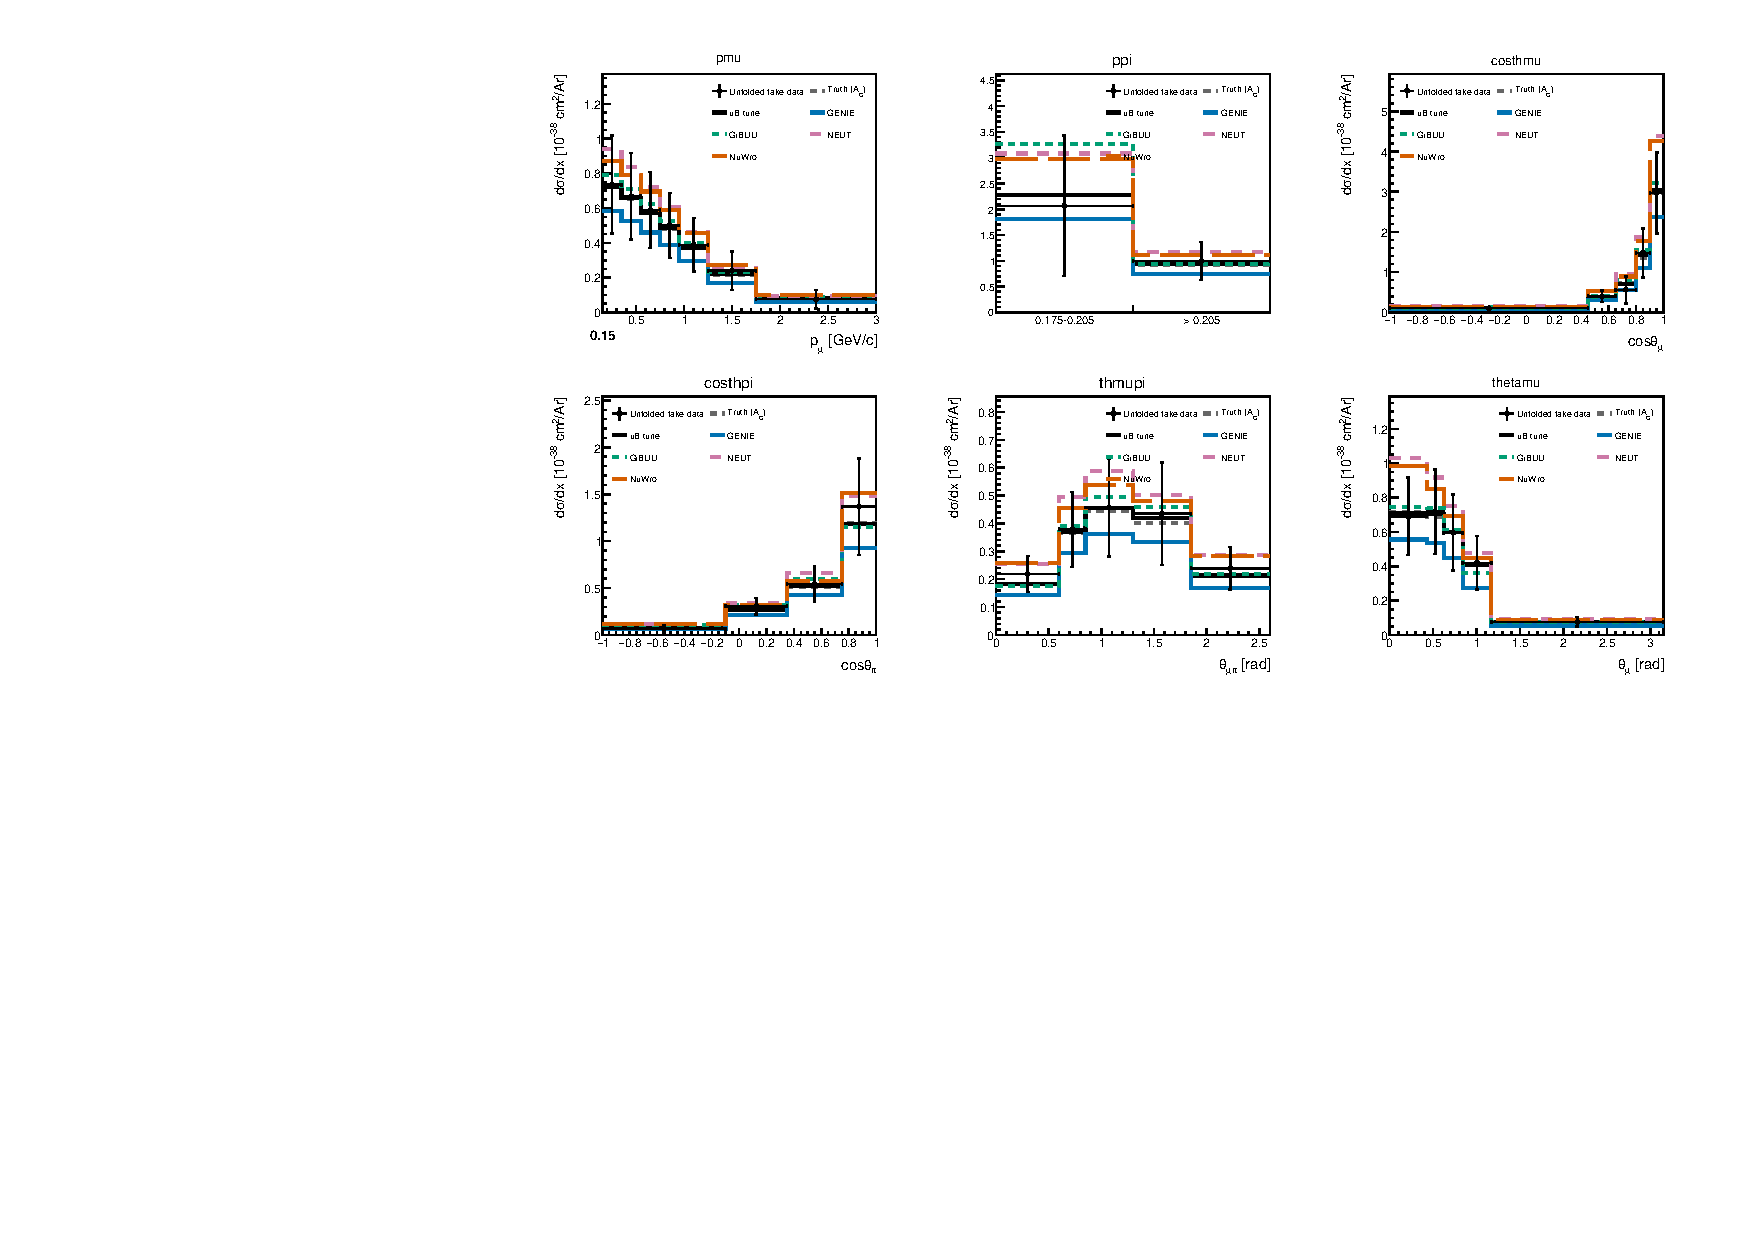
\includegraphics[width=0.98\textwidth]{dsigma_FHC5}
  \caption{FHC differential cross sections in the six released distributions. Points are the
    unfolded data with the total uncertainty; the grey dashed histogram is the $\AC$-smeared
    central-value truth, the black histogram the \uboone{} tune, and the coloured histograms GENIE,
    GiBUU, NEUT and NuWro, all multiplied by $\AC$. [DRAFT: blind fake data.]}
  \label{fig:fhc}
\end{figure*}
\begin{figure*}[t]
  \centering
  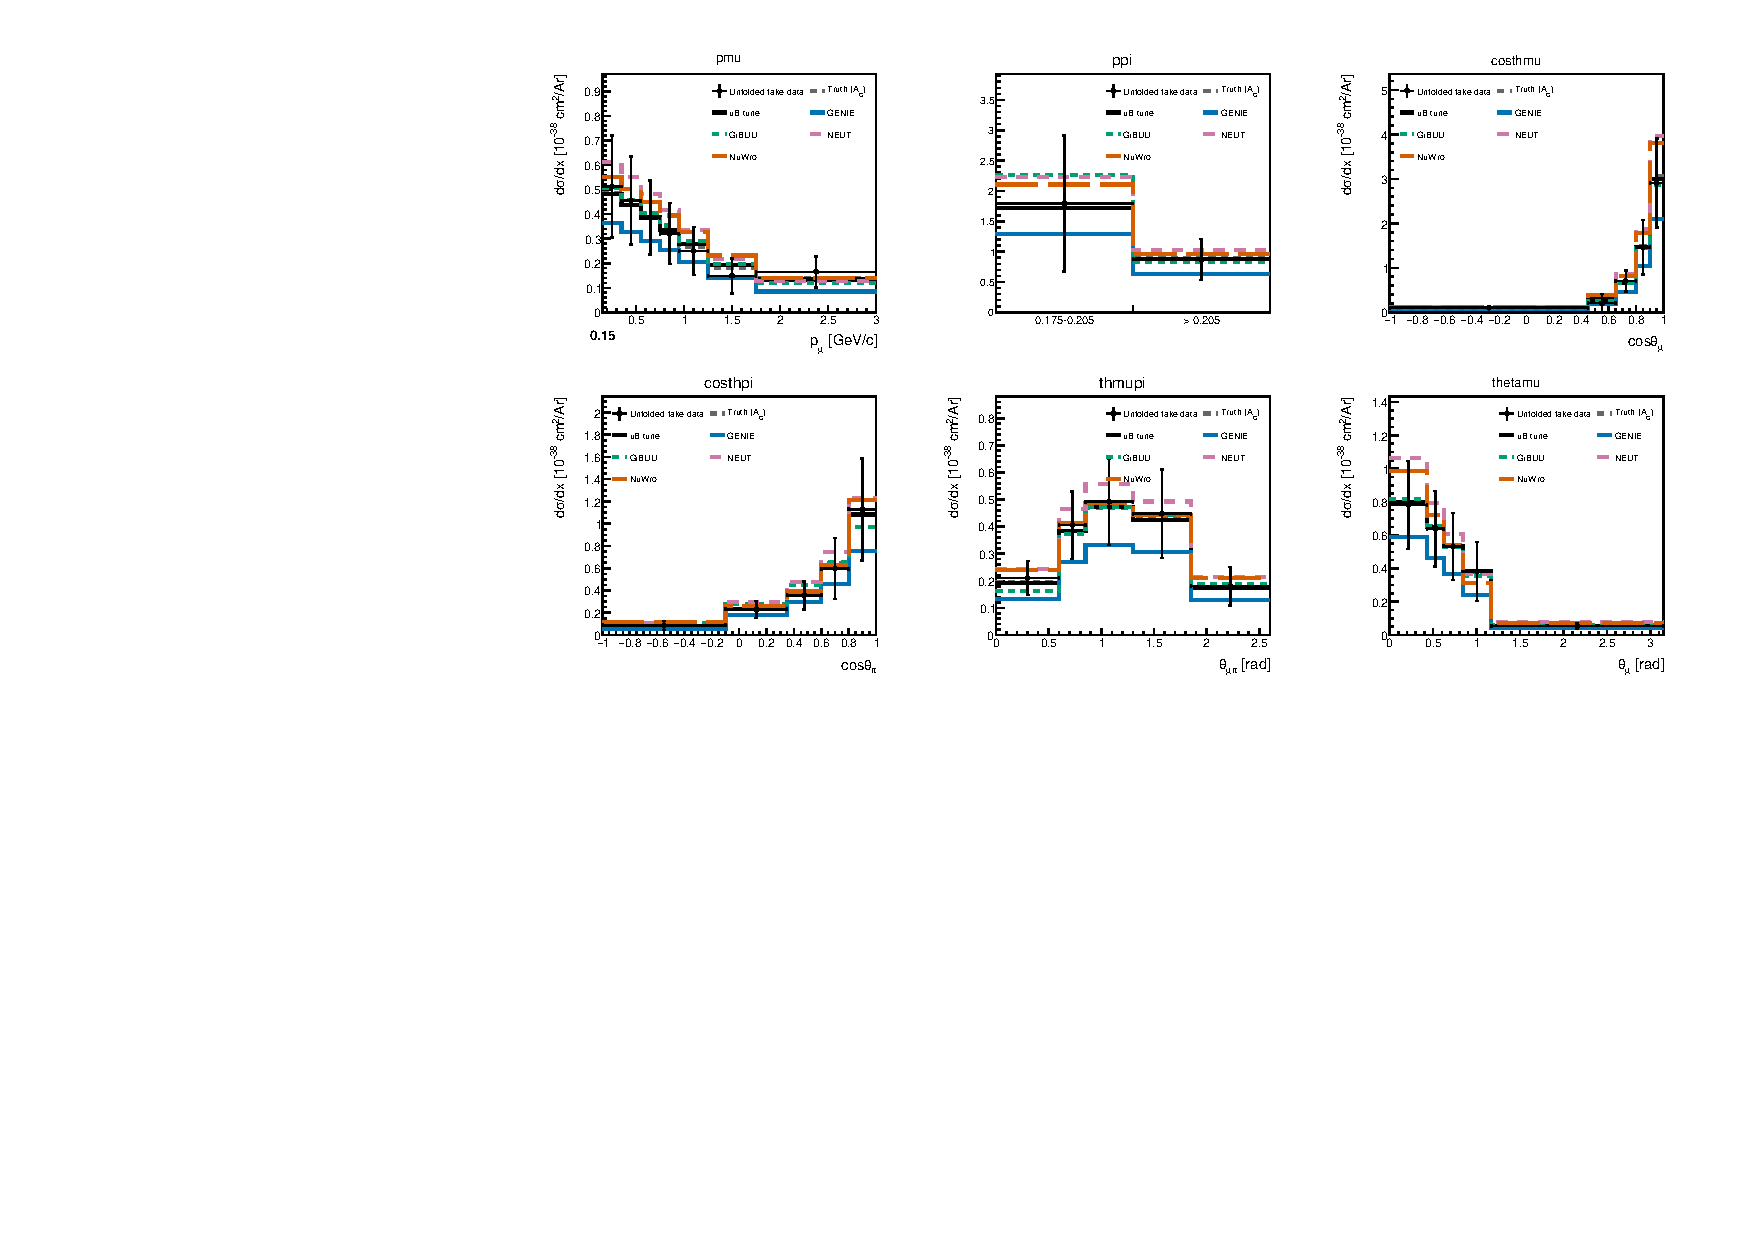
\includegraphics[width=0.98\textwidth]{dsigma_RHCFULL}
  \caption{As Fig.~\ref{fig:fhc}, for RHC.}
  \label{fig:rhc}
\end{figure*}
\begin{figure*}[t]
  \centering
  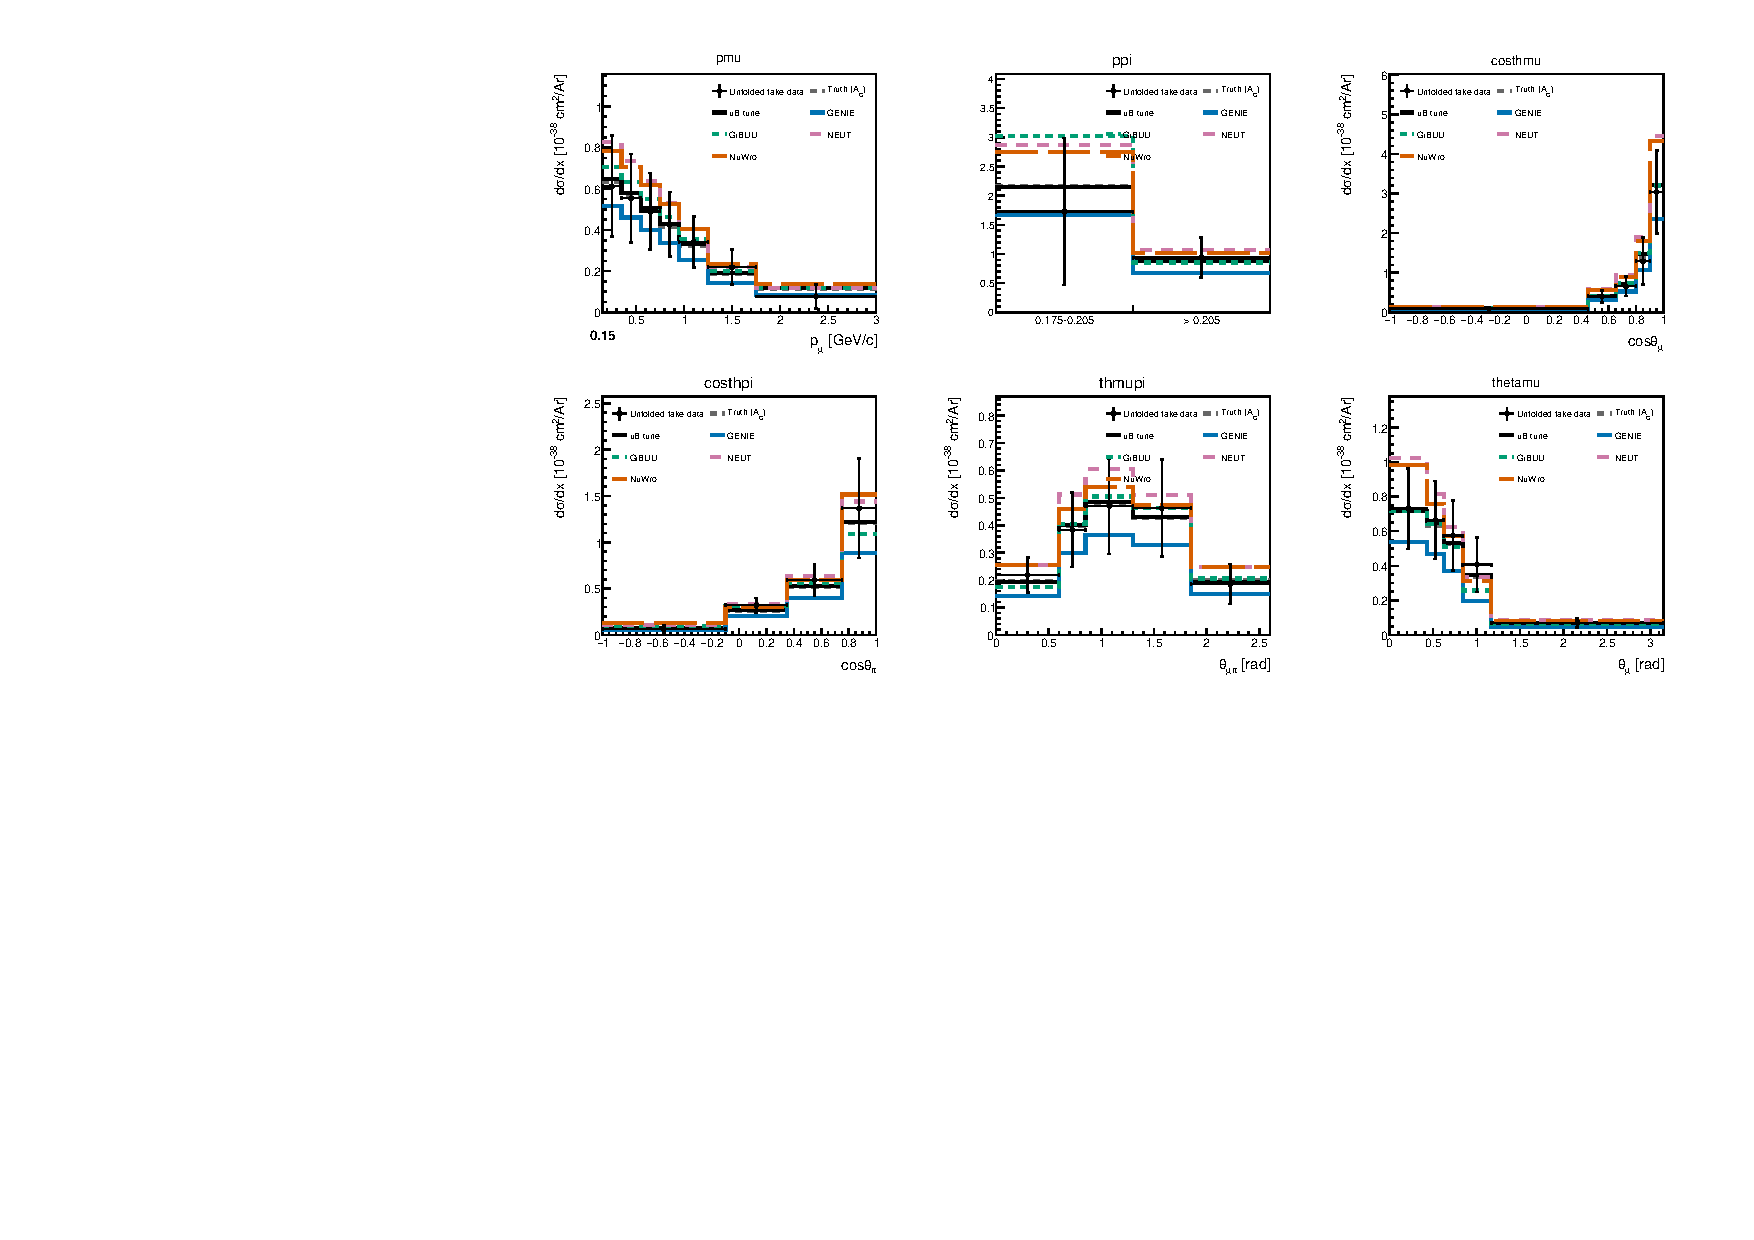
\includegraphics[width=0.98\textwidth]{dsigma_COMB}
  \caption{As Fig.~\ref{fig:fhc}, for the combined configuration.}
  \label{fig:comb}
\end{figure*}

Figures~\ref{fig:fhc}--\ref{fig:comb} show the six differential distributions in each
configuration. The muon polar angle is released in both $\cos\theta_\mu$ and $\theta_\mu$; the
two are separate extractions with different responses, not a change of variable, and the
$\theta_\mu$ response is the better conditioned of the two. The muon--pion opening angle is the
best-conditioned shape observable. In every distribution the generators differ mainly in
normalisation, with the largest shape differences in the forward $\cos\theta_\pi$ bins and the
high-momentum $p_\mu$ tail.

\subsection{The two-region pion momentum}

The upper pion-momentum region, $p_\pi>0.205\GeVc$, is open-ended and has no width; it therefore
has no differential density, and the $p_\pi$ result is quoted as two bin-integrated cross
sections (Table~\ref{tab:ppi}). The differential form in the figures uses a reporting width of
$0.795\GeVc$ for the upper region so that it can be drawn on the same axis as the first, and a
height read from it is that convention rather than a measurement.

\begin{table}[t]
  \caption{The $p_\pi$ result as bin integrals, $10^{-38}$~cm$^2$/Ar. [DRAFT: blind placeholders.]}
  \label{tab:ppi}
  \begin{ruledtabular}
  \begin{tabular}{lccc}
    Region & FHC & RHC & Combined \\
    \hline
    $0.175<p_\pi<0.205\GeVc$ & $0.059\pm0.041$ & $0.054\pm0.034$ & $0.062\pm0.038$ \\
    $p_\pi>0.205\GeVc$ & $0.764\pm0.293$ & $0.694\pm0.268$ & $0.713\pm0.270$ \\
  \end{tabular}
  \end{ruledtabular}
\end{table}

\section{Limitations}
\label{sec:limitations}

The following are identified but not in the released covariance: a dedicated systematic on the
multiple-Coulomb-scattering momentum scale and resolution, which $63\%$ of selected FHC muons rely
on; an uncertainty on the beam-off gate ratios; and the use of the Run-1 beam-off sample in place
of a dedicated Run-2 one. The statistical-coverage and alternative-model tests were run for FHC and
have not yet been extended to RHC. These are stated so that the covariance is read as what it is:
complete with respect to the nominal configured uncertainty model.

\section{Conclusions}

We have measured the flux-averaged total and six differential cross sections for
$\nu_\mu+\bar\nu_\mu$ charged-current single charged-pion production on argon with the full
\uboone{} NuMI exposure in forward-horn, reverse-horn and combined configurations, with every
angle defined about the neutrino direction. The extraction is validated in its implementation, its
statistical uncertainties and its robustness to a wrong interaction model, and the background model
is confirmed in beam-on control regions. The additional-smearing matrices and covariances for every
result are released, and are required to compare any prediction with them. The kinematics of the
hadronic system in the proton-tagged subsample are reported in a companion Letter.

\begin{acknowledgments}
[Standard \uboone{} acknowledgments.]
\end{acknowledgments}

\appendix
\section{Bin edges}
The released binnings are: $p_\mu$ [GeV/$c$] $0.15,0.35,0.55,0.75,0.95,1.25,1.75,3$;
$p_\pi$ [GeV/$c$] $0.175,0.205,\infty$; $\cos\theta_\mu$ $-1,0.45,0.65,0.8,0.9,1$;
$\theta_\mu$ [rad] $0,0.43,0.62,0.84,1.17,\pi$; $\cos\theta_\pi$ $-1,-0.1,0.35,0.6,0.8,1$;
$\theta_{\mu\pi}$ [rad] $0,0.6,0.85,1.3,1.85,2.6$.

\section{Using the released matrices}
For a prediction $P_j$ in the true bins of an observable, the comparable quantity is
$(\AC P)_i$, and the $\chi^2$ against the unfolded result $D_i$ is
$(D-\AC P)^T\,{\rm Cov}^{-1}\,(D-\AC P)$ with the released covariance. Neither step can be omitted.

\begin{thebibliography}{99}

\bibitem{numi_nue_ccpi}
  MicroBooNE Collaboration,
  ``Measurement of the flux-averaged differential $\nu_e$ CC$1\pi$ cross section
  in the NuMI beam,'' Internal Note v3.2 (2025).

\bibitem{mistry_thesis}
  K.~Mistry,
  ``First Measurement of the Flux-Averaged Differential Charged-Current
  Electron-Neutrino and Antineutrino Cross Section on Argon with the MicroBooNE
  Detector,'' PhD thesis (2021).

\bibitem{nova}
  NOvA Collaboration, M.~A.~Acero \textit{et al.},
  ``New constraints on oscillation parameters from $\nu_e$ appearance and
  $\nu_\mu$ disappearance in the NOvA experiment,''
  \textit{Phys.\ Rev.\ D} \textbf{98}, 032012 (2018).

\bibitem{t2k}
  T2K Collaboration, K.~Abe \textit{et al.},
  ``Constraint on the matter--antimatter symmetry-violating phase in neutrino
  oscillations,''
  \textit{Nature} \textbf{580}, 339--344 (2020).

\bibitem{dune}
  DUNE Collaboration, B.~Abi \textit{et al.},
  ``Deep Underground Neutrino Experiment (DUNE), Far Detector Technical Design
  Report, Volume II: DUNE Physics,'' arXiv:2002.03005 [hep-ex] (2020).

\bibitem{pandora}
  J.~S.~Marshall and M.~A.~Thomson,
  ``The Pandora Software Development Kit for Pattern Recognition,''
  \textit{Eur.\ Phys.\ J.\ C} \textbf{75}, 439 (2015).

\bibitem{wienervsd}
  W.~Tang, X.~Li, X.~Qian, H.~Wei, and C.~Zhang,
  ``Data Unfolding with Wiener-SVD Method,''
  \textit{JINST} \textbf{12}, P10002 (2017), arXiv:1705.03568 [physics.data-an].

\bibitem{ppfx}
  L.~Aliaga \textit{et al.}\ (MINERvA Collaboration),
  ``Neutrino Flux Predictions for the NuMI Beam,''
  \textit{Phys.\ Rev.\ D} \textbf{94}, 092005 (2016).

\bibitem{genie}
  C.~Andreopoulos \textit{et al.},
  ``The GENIE Neutrino Monte Carlo Generator,''
  \textit{Nucl.\ Instrum.\ Methods A} \textbf{614}, 87--104 (2010).

\bibitem{sce}
  MicroBooNE Collaboration, P.~Abratenko \textit{et al.},
  ``Measurement of space charge effects in the MicroBooNE LArTPC using cosmic
  muons,''
  \textit{JINST} \textbf{15}, P12037 (2020).

\bibitem{uboone_laser}
  MicroBooNE Collaboration, C.~Adams \textit{et al.},
  ``A Method to Determine the Electric Field of Liquid Argon Time Projection
  Chambers Using a UV Laser System and Its Application in MicroBooNE,''
  \textit{JINST} \textbf{15}, P07010 (2020).

\bibitem{uboone_pandora}
  MicroBooNE Collaboration, R.~Acciarri \textit{et al.},
  ``The Pandora multi-algorithm approach to automated pattern recognition of
  cosmic-ray muon and neutrino events in the MicroBooNE detector,''
  \textit{Eur.\ Phys.\ J.\ C} \textbf{78}, 82 (2018).

\bibitem{uboone_llr}
  MicroBooNE Collaboration, P.~Abratenko \textit{et al.},
  ``Calorimetric classification of track-like signatures in liquid argon TPCs
  using MicroBooNE data,''
  \textit{JHEP} \textbf{12}, 153 (2021).

\bibitem{uboone_mcs}
  MicroBooNE Collaboration, P.~Abratenko \textit{et al.},
  ``Determination of muon momentum in the MicroBooNE LArTPC using an improved
  model of multiple Coulomb scattering,''
  \textit{JINST} \textbf{12}, P10010 (2017).

\bibitem{uboone_detvar}
  MicroBooNE Collaboration, P.~Abratenko \textit{et al.},
  ``Novel approach for evaluating detector-related uncertainties in a LArTPC
  using MicroBooNE data,''
  \textit{Eur.\ Phys.\ J.\ C} \textbf{82}, 454 (2022).

\bibitem{uboone_tune}
  MicroBooNE Collaboration, P.~Abratenko \textit{et al.},
  ``New CC0$\pi$ GENIE model tune for MicroBooNE,''
  \textit{Phys.\ Rev.\ D} \textbf{105}, 072001 (2022), arXiv:2110.14028 [hep-ex].

\bibitem{uboone_tki}
  MicroBooNE Collaboration, P.~Abratenko \textit{et al.},
  ``First double-differential measurement of kinematic imbalance in neutrino
  interactions with the MicroBooNE detector,''
  \textit{Phys.\ Rev.\ Lett.} \textbf{131}, 101802 (2023), arXiv:2301.03700 [hep-ex].

\bibitem{xsec_analyzer}
  S.~Gardiner \textit{et al.},
  ``XSecAnalyzer: a cross-section analysis framework for MicroBooNE,''
  \url{https://github.com/uboone/xsec_analyzer} (accessed 2026).

\bibitem{numi_beam}
  P.~Adamson \textit{et al.},
  ``The NuMI Neutrino Beam,''
  \textit{Nucl.\ Instrum.\ Methods A} \textbf{806}, 279--306 (2016).

\bibitem{genie3}
  L.~Alvarez-Ruso \textit{et al.}\ (GENIE Collaboration),
  ``Recent highlights from GENIE v3,''
  \textit{Eur.\ Phys.\ J.\ ST} \textbf{230}, 4449--4467 (2021).

\bibitem{nuwro}
  T.~Golan, J.~T.~Sobczyk, and J.~\.Zmuda,
  ``NuWro: the Wroc\l{}aw Monte Carlo generator of neutrino interactions,''
  \textit{Nucl.\ Phys.\ B Proc.\ Suppl.} \textbf{229--232}, 499 (2012).

\bibitem{gibuu}
  O.~Buss \textit{et al.},
  ``Transport-theoretical description of nuclear reactions,''
  \textit{Phys.\ Rept.} \textbf{512}, 1--124 (2012);
  U.~Mosel, ``Neutrino event generators: foundation, status and future,''
  \textit{J.\ Phys.\ G} \textbf{46}, 113001 (2019).

\bibitem{neut2021}
  Y.~Hayato and L.~Pickering,
  ``The NEUT neutrino interaction simulation program library,''
  \textit{Eur.\ Phys.\ J.\ ST} \textbf{230}, 4469--4481 (2021).

\bibitem{geant4}
  S.~Agostinelli \textit{et al.}\ (GEANT4 Collaboration),
  ``GEANT4: a simulation toolkit,''
  \textit{Nucl.\ Instrum.\ Methods A} \textbf{506}, 250--303 (2003).

\bibitem{geant4reweight}
  J.~Calcutt, C.~Thorpe, K.~Mahn, and L.~Fields,
  ``Geant4Reweight: a framework for evaluating and propagating hadronic
  interaction uncertainties in Geant4,''
  \textit{JINST} \textbf{16}, P08042 (2021).

\bibitem{tmva}
  A.~Hoecker \textit{et al.},
  ``TMVA: Toolkit for Multivariate Data Analysis,''
  PoS \textbf{ACAT}, 040 (2007), arXiv:physics/0703039.

\bibitem{dagostini}
  G.~D'Agostini,
  ``A multidimensional unfolding method based on Bayes' theorem,''
  \textit{Nucl.\ Instrum.\ Methods A} \textbf{362}, 487--498 (1995).

\bibitem{lu_tki}
  X.-G.~Lu, L.~Pickering, S.~Dolan, G.~Barr, D.~Coplowe, Y.~Uchida, D.~Wark,
  M.~O.~Wascko, A.~Weber, and T.~Yuan,
  ``Measurement of nuclear effects in neutrino interactions with minimal
  dependence on neutrino energy,''
  \textit{Phys.\ Rev.\ C} \textbf{94}, 015503 (2016).

\bibitem{furmanski_pn}
  A.~P.~Furmanski and J.~T.~Sobczyk,
  ``Neutrino energy reconstruction from one-muon and one-proton events,''
  \textit{Phys.\ Rev.\ C} \textbf{95}, 065501 (2017).

\bibitem{rs_coherent}
  D.~Rein and L.~M.~Sehgal,
  ``Coherent $\pi^0$ production in neutrino reactions,''
  \textit{Nucl.\ Phys.\ B} \textbf{223}, 29--44 (1983).

\bibitem{berger_sehgal_coherent}
  C.~Berger and L.~M.~Sehgal,
  ``Partially conserved axial vector current and coherent pion production by
  low energy neutrinos,''
  \textit{Phys.\ Rev.\ D} \textbf{79}, 053003 (2009).

\bibitem{genieccpi}
  MicroBooNE Collaboration, P.~Abratenko \textit{et al.},
  ``First Measurement of Energy-Dependent Inclusive Muon-Neutrino
  Charged-Current Cross Sections on Argon with the MicroBooNE Detector,''
  \textit{Phys.\ Rev.\ Lett.} \textbf{128}, 151801 (2022), arXiv:2110.14023 [hep-ex].

\bibitem{uboone_nim}
  MicroBooNE Collaboration, R.~Acciarri \textit{et al.},
  ``Design and Construction of the MicroBooNE Detector,''
  \textit{JINST} \textbf{12}, P02017 (2017).

\bibitem{uboone_crt}
  MicroBooNE Collaboration, C.~Adams \textit{et al.},
  ``Design and construction of the MicroBooNE Cosmic Ray Tagger system,''
  \textit{JINST} \textbf{14}, P04004 (2019).

\bibitem{rs1981}
  D.~Rein and L.~M.~Sehgal,
  ``Neutrino Excitation of Baryon Resonances and Single Pion Production,''
  \textit{Ann.\ Phys.} \textbf{133}, 79--153 (1981).

\bibitem{kuzmin2004}
  K.~S.~Kuzmin, V.~V.~Lyubushkin, and V.~A.~Naumov,
  ``Lepton polarization in neutrino nucleon interactions,''
  \textit{Mod.\ Phys.\ Lett.\ A} \textbf{19}, 2815--2829 (2004).

\bibitem{graczyk2008}
  K.~M.~Graczyk and J.~T.~Sobczyk,
  ``Form factors in the quark resonance model,''
  \textit{Phys.\ Rev.\ D} \textbf{77}, 053001 (2008)
  [Erratum: \textit{Phys.\ Rev.\ D} \textbf{79}, 079903 (2009)].

\bibitem{berger2007}
  C.~Berger and L.~Sehgal,
  ``Lepton mass effects in single pion production by neutrinos,''
  \textit{Phys.\ Rev.\ D} \textbf{76}, 113004 (2007).

\bibitem{nowak2009}
  J.~A.~Nowak (MiniBooNE Collaboration),
  ``Four-momentum transfer discrepancy in the charged current $\pi^+$ production
  in the MiniBooNE: Data vs.\ theory,''
  \textit{AIP Conf.\ Proc.} \textbf{1189}, 243--248 (2009).

\bibitem{neut}
  Y.~Hayato,
  ``A neutrino interaction simulation program library NEUT,''
  \textit{Acta Phys.\ Polon.\ B} \textbf{40}, 2477--2489 (2009).

\bibitem{anl_radecky1982}
  G.~M.~Radecky \textit{et al.}\ (ANL Collaboration),
  ``Study of single pion production by weak charged currents in low-energy
  $\nu d$ interactions,''
  \textit{Phys.\ Rev.\ D} \textbf{25}, 1161--1173 (1982).

\bibitem{bnl_kitagaki1986}
  T.~Kitagaki \textit{et al.}\ (BNL Collaboration),
  ``Charged-current exclusive pion production in neutrino--deuterium
  interactions,''
  \textit{Phys.\ Rev.\ D} \textbf{34}, 2554--2565 (1986).

\bibitem{k2k_rodriguez2008}
  A.~Rodriguez \textit{et al.}\ (K2K Collaboration),
  ``Measurement of single charged pion production in the charged-current
  interactions of neutrinos in a 1.3~GeV wide band beam,''
  \textit{Phys.\ Rev.\ D} \textbf{78}, 032003 (2008).

\bibitem{miniboone_ccpi}
  A.~A.~Aguilar-Arevalo \textit{et al.}\ (MiniBooNE Collaboration),
  ``Measurement of $\nu_\mu$-induced charged-current single positive pion
  production cross sections on mineral oil at $E_\nu \in 0.5$--$2.0$~GeV,''
  \textit{Phys.\ Rev.\ D} \textbf{83}, 052007 (2011).

\bibitem{minerva_tki}
  X.-G.~Lu \textit{et al.}\ (MINERvA Collaboration),
  ``Measurement of final-state correlations in neutrino muon-proton mesonless
  production on hydrocarbon at $\langle E_\nu\rangle=3$~GeV,''
  Phys.\ Rev.\ Lett.\ \textbf{121}, 022504 (2018).

\bibitem{minerva_ccpi}
  B.~Eberly \textit{et al.}\ (MINERvA Collaboration),
  ``Charged pion production in $\nu_\mu$ interactions on hydrocarbon at
  $\langle E_\nu \rangle = 4.0$~GeV,''
  \textit{Phys.\ Rev.\ D} \textbf{92}, 092008 (2015).

\bibitem{minerva_fe}
  C.~L.~McGivern \textit{et al.}\ (MINERvA Collaboration),
  ``Cross sections for $\nu_\mu$ and $\bar{\nu}_\mu$ induced pion production on
  hydrocarbon in the few-GeV region using MINERvA,''
  \textit{Phys.\ Rev.\ D} \textbf{94}, 052005 (2016).

\bibitem{minerva_lownu}
  MINERvA Collaboration, J.~Wolcott \textit{et al.},
  ``Evidence for Quasielastic Charge Current Antineutrino Scattering Off
  Protons in Hydrocarbon at $\langle E_{\bar\nu} \rangle = 3.5$~GeV,''
  \textit{Phys.\ Rev.\ Lett.} \textbf{116}, 081802 (2016).

\bibitem{t2k_ccpip}
  K.~Abe \textit{et al.}\ (T2K Collaboration),
  ``Measurement of the muon neutrino charged-current single $\pi^+$ production
  on hydrocarbon using the T2K off-axis near detector ND280,''
  \textit{Phys.\ Rev.\ D} \textbf{101}, 012007 (2020), arXiv:1909.03936 [hep-ex].

\bibitem{argoneut_ccpi}
  R.~Acciarri \textit{et al.}\ (ArgoNEUT Collaboration),
  ``First measurement of the cross section for $\nu_\mu$ and $\bar{\nu}_\mu$
  induced single charged pion production on argon using ArgoNEUT,''
  \textit{Phys.\ Rev.\ D} \textbf{98}, 052002 (2018), arXiv:1804.10294 [hep-ex].

\bibitem{uboone_nue_ccpi}
  MicroBooNE Collaboration, P.~Abratenko \textit{et al.},
  ``First measurement of $\nu_e$ and $\bar{\nu}_e$ charged-current single
  charged-pion production differential cross sections on argon using the
  MicroBooNE detector,''
  \textit{Phys.\ Rev.\ Lett.} \textbf{135}, 061802 (2025),
  arXiv:2503.23384 [hep-ex].

\bibitem{uboone_bnb2026_ccpi}
  MicroBooNE Collaboration, P.~Abratenko \textit{et al.},
  ``Measurement of single charged pion production in charged-current
  $\nu_\mu$-Ar interactions with the MicroBooNE detector,''
  \textit{Phys.\ Rev.\ D} \textbf{113}, 032007 (2026),
  arXiv:2509.03628 [hep-ex].


\bibitem{companion_prd} \uboone{} Collaboration, ``Measurement of $\nu_\mu$ and $\bar\nu_\mu$
  charged-current single charged-pion production differential cross sections on argon in the NuMI
  beam,'' companion article, submitted to Phys.\ Rev.\ D (joint submission).
\bibitem{t2k_tki} K.~Abe \emph{et al.} (T2K Collaboration), ``Characterization of nuclear effects
  in muon-neutrino scattering on hydrocarbon with a measurement of final-state kinematics and
  correlations in charged-current pionless interactions at T2K,'' Phys.\ Rev.\ D \textbf{98},
  032003 (2018).
\bibitem{companion_prl} \uboone{} Collaboration, ``First measurement of transverse kinematic
  imbalance and hadronic-system kinematics in charged-current single-pion production on argon,''
  companion Letter, submitted to Phys.\ Rev.\ Lett.\ (joint submission).
\end{thebibliography}


\end{document}
